\chapter{Results}
\label{chap:results}

This chapter begins with a validation experiment that confirms the correctness of my quantum implementation (Section~\ref{sec:res_validation}), then presents the main results for standard classification (Section~\ref{sec:res_standard}) and zero-day attack detection (Section~\ref{sec:res_zeroday}). Section~\ref{sec:res_sensitivity} analyzes parameter initialization sensitivity, Section~\ref{sec:res_training} discusses training dynamics and ablation studies, and Section~\ref{sec:res_discussion} summarizes the findings. All quantum results are averaged over 10~random seeds; the autoencoder is also evaluated on 10~seeds. A consolidated table of all results is provided in Appendix~\ref{app:full_results}.

% ============================================================
\section{Implementation Validation}
\label{sec:res_validation}

Before evaluating on the IoT dataset, I validate the data re-uploading implementation on two standard synthetic benchmarks from the literature. P\'erez-Salinas et al.~\cite{perez2020data} report 90--98\% accuracy on similar 2D classification tasks. I train a single-qubit re-uploading circuit (4~layers, 24~parameters) for 80~epochs on 300~training samples from \texttt{make\_circles} and \texttt{make\_moons} (scikit-learn). Table~\ref{tab:res_validation} reports the results.

\begin{table}[ht]
\centering
\begin{tabular}{lccccc}
    \toprule
    \textbf{Dataset} & \textbf{Params} & \textbf{Accuracy} & \textbf{F1} & \textbf{MCC} \\
    \midrule
    \texttt{make\_circles} & 24 & 0.990 & 0.990 & 0.980 \\
    \texttt{make\_moons}   & 24 & 1.000 & 1.000 & 1.000 \\
    \bottomrule
\end{tabular}
\caption{Validation results on synthetic 2D datasets. My implementation achieves 99--100\% accuracy, consistent with the 90--98\% range reported by P\'erez-Salinas et al.~\cite{perez2020data}, confirming that the quantum circuit and training pipeline are correctly implemented.}
\label{tab:res_validation}
\end{table}

% ============================================================
\section{Standard Classification}
\label{sec:res_standard}

Table~\ref{tab:res_standard} reports accuracy, weighted F1-score, and Matthews Correlation Coefficient (MCC) on the 200-sample test set for the standard 3-class setting. MCC is included as it provides a balanced measure even when class sizes differ slightly~\cite{chicco2020advantages}. Quantum results are reported as mean~$\pm$~standard deviation over 10~random seeds (see Section~\ref{sec:res_sensitivity}).

\begin{table}[ht]
\centering
\begin{tabular}{llccc}
    \toprule
    \textbf{Model} & \textbf{Type} & \textbf{Accuracy} & \textbf{F1} & \textbf{MCC} \\
    \midrule
    Random Forest          & Classical & 0.990 & 0.990 & 0.985 \\
    SVM (RBF)              & Classical & 0.970 & 0.970 & 0.955 \\
    NN-Medium (16,\,8)     & Classical & 0.960 & 0.960 & 0.940 \\
    NN-Small (12,\,6)      & Classical & 0.925 & 0.925 & 0.888 \\
    \midrule
    Re-uploading 1q        & Quantum   & 0.752 $\pm$ 0.039 & 0.720 $\pm$ 0.051 & 0.662 $\pm$ 0.045 \\
    Re-uploading 4q        & Quantum   & 0.692 $\pm$ 0.011 & 0.654 $\pm$ 0.010 & 0.586 $\pm$ 0.016 \\
    QCNN (8q)              & Quantum   & 0.679 $\pm$ 0.025 & 0.636 $\pm$ 0.021 & 0.559 $\pm$ 0.043 \\
    \bottomrule
\end{tabular}
\caption{Standard 3-class results (normal / DoS / injection). Classical models are trained on 500 quantum-subset samples and tested on 200 samples. Quantum results are mean $\pm$ std over 10 seeds.}
\label{tab:res_standard}
\end{table}

All classical models achieve high accuracy ($\geq 92.5\%$), indicating strong class separation in the selected features. The quantum models perform significantly worse: the best quantum result is the single-qubit re-uploading at 75.2\% accuracy (MCC 0.66). The QCNN achieves 67.9\% with an MCC of 0.56.

These classical results are consistent with prior evaluations of ML models on ToN\_IoT: Moustafa~\cite{moustafa2021toniot} reports that tree-based and kernel methods consistently achieve $>$95\% accuracy on this dataset, confirming that our preprocessing pipeline and baseline implementation are correct.

This gap between classical and quantum is consistent with prior work showing that quantum classifiers do not outperform classical methods on datasets that are already linearly or near-linearly separable in the original feature space~\cite{schuld2021effect, bowles2024better}. With 8~well-chosen features, a Random Forest achieves 99\% accuracy with only 500~training samples, leaving no room for quantum advantage on this task.

% ============================================================
\section{Zero-Day Attack Detection}
\label{sec:res_zeroday}

Table~\ref{tab:res_zeroday} reports results on the zero-day setting, where models are trained exclusively on normal and DoS traffic and then tested on injection attacks---a class entirely absent from training. Since the test set is homogeneous (all injection), I report accuracy as the primary metric (equivalent to recall for the attack class). Quantum and autoencoder results are mean~$\pm$~std over 10~seeds.

\begin{table}[ht]
\centering
\begin{tabular}{llcc}
    \toprule
    \textbf{Model} & \textbf{Type} & \textbf{Accuracy} & \textbf{F1} \\
    \midrule
    Autoencoder (anomaly detection)        & Classical & \textbf{0.705 $\pm$ 0.144} & \textbf{0.819 $\pm$ 0.100} \\
    QCNN (8q), excl.\ barren-plateau seeds & Quantum   & \textbf{0.686 $\pm$ 0.068} & \textbf{0.812 $\pm$ 0.051} \\
    QCNN (8q), all 10 seeds                & Quantum   & 0.490 $\pm$ 0.305          & 0.587 $\pm$ 0.349 \\
    Re-uploading 1q                        & Quantum   & 0.092 $\pm$ 0.036          & 0.167 $\pm$ 0.058 \\
    Re-uploading 4q                        & Quantum   & 0.075 $\pm$ 0.023          & 0.138 $\pm$ 0.039 \\
    \midrule
    NN-Small (12,\,6)      & Classical & 0.028 & 0.054 \\
    SVM (RBF)              & Classical & 0.024 & 0.046 \\
    NN-Medium (16,\,8)     & Classical & 0.017 & 0.034 \\
    Random Forest          & Classical & 0.003 & 0.007 \\
    \bottomrule
\end{tabular}
\caption{Zero-day detection results. Models are trained on normal + DoS only; the test set contains exclusively injection attacks (unseen during training). Supervised classical models are evaluated on the full zero-day test set (7,034 samples); the autoencoder uses the same 7,034 samples as test set and is trained on all ${\sim}28{,}000$ normal samples; quantum models use a 200-sample test subsample and 500 training samples due to simulation cost. Autoencoder and quantum results are mean $\pm$ std over 10 seeds. The ``excl.\ barren-plateau seeds'' row reports the mean over the 7 seeds for which the QCNN converges; the 3 collapsed seeds $\{2, 5, 6\}$ (zero-day detection $\leq 9\%$) are excluded. Per-seed values are given in Table~\ref{tab:res_seeds} (Section~\ref{sec:res_sensitivity}).}
\label{tab:res_zeroday}
\end{table}

The results separate the seven evaluated models into three regimes:

\textbf{Supervised classical models fail completely.} Every supervised classical baseline (Random Forest, SVM, NN-Small, NN-Medium) detects fewer than 3\% of injection attacks. This is the expected behaviour: a classifier trained to discriminate \emph{normal} from \emph{DoS} learns a boundary tuned to those two distributions, and an unseen attack class lying away from that boundary is silently absorbed into one of the known classes.

\textbf{Two approaches reach $\sim$70\%.} The autoencoder (70.5\% $\pm$ 14.4\%) and the QCNN excluding barren-plateau seeds (68.6\% $\pm$ 6.8\%) reach essentially the same mean detection rate, an order of magnitude above the supervised classical baselines---but they are not both unsupervised. The autoencoder is trained on normal traffic only and flags any input that does not reconstruct well (genuine unsupervised anomaly detection). The QCNN is trained \emph{supervised} on normal-vs-DoS labels and happens to transfer to injection on 7 out of 10 initializations, suggesting that its quantum feature map captures a broader notion of ``not normal'' rather than memorizing the DoS distribution. Both approaches share the underlying intuition of modelling normal traffic and treating anything anomalous as an attack, but reach it through fundamentally different training regimes.

\textbf{Re-uploading remains brittle on zero-day.} Both re-uploading variants stay at 7--9\% on injection (versus ${\sim}2$--$3$\% for supervised classical), indicating they generalize slightly beyond their training classes but fall well short of the QCNN and the autoencoder. Their flatter feature maps appear to fit the specific DoS distribution rather than learning a broader notion of ``normal'' versus ``attack''.

The QCNN's headline number depends critically on whether barren-plateau seeds are included: across all 10 seeds the mean is 49.0\% with a 30.5\% standard deviation, masking a bimodal behaviour with 7~successful runs (54--76\%) and 3~training collapses ($\leq 9\%$). Section~\ref{sec:res_sensitivity} returns to this point. The autoencoder is more stable across seeds in terms of failure rate (1/10 vs.\ 3/10), but its detection rate when training succeeds varies more (std 14.4\% vs.\ 6.8\% for the QCNN).

A methodological note. The autoencoder is trained on all ${\sim}28{,}000$ normal samples while the quantum classifiers are restricted to the 500-sample quantum subsample for simulation-cost reasons (Chapter~\ref{chap:dataset}). The two methods therefore see different amounts of data, and this asymmetry should temper any direct numerical comparison. It does not, however, change the qualitative ranking observed: supervised classical $\ll$ re-uploading $<$ \{autoencoder, QCNN\}.

% ============================================================
\section{Initialization Sensitivity Analysis}
\label{sec:res_sensitivity}

The large standard deviation observed in QCNN zero-day performance motivated a systematic analysis of parameter initialization sensitivity. Table~\ref{tab:res_seeds} shows the per-seed QCNN results on the zero-day task (500 training samples, 100 epochs, 10 seeds).

\begin{table}[ht]
\centering
\begin{tabular}{lcccc}
    \toprule
    \textbf{Seed} & \textbf{Std.\ Acc.} & \textbf{Std.\ F1} & \textbf{ZD Acc.} & \textbf{ZD F1} \\
    \midrule
    0 & 0.720 & 0.674 & 0.755 & 0.860 \\
    1 & 0.675 & 0.638 & 0.640 & 0.780 \\
    2 & 0.625 & 0.593 & \textit{0.010} & \textit{0.020} \\
    3 & 0.685 & 0.616 & 0.730 & 0.844 \\
    4 & 0.680 & 0.641 & 0.695 & 0.820 \\
    5 & 0.690 & 0.650 & \textit{0.000} & \textit{0.000} \\
    6 & 0.665 & 0.629 & \textit{0.090} & \textit{0.165} \\
    7 & 0.680 & 0.642 & 0.710 & 0.830 \\
    8 & 0.660 & 0.625 & 0.730 & 0.844 \\
    9 & 0.710 & 0.651 & 0.540 & 0.701 \\
    \midrule
    Mean $\pm$ std (all 10)         & 0.679 $\pm$ 0.025 & 0.636 $\pm$ 0.021 & 0.490 $\pm$ 0.305 & 0.587 $\pm$ 0.349 \\
    Mean (excl.\ barren: 2,5,6) & 0.687 $\pm$ 0.019 & 0.641 $\pm$ 0.017 & 0.686 $\pm$ 0.068 & 0.812 $\pm$ 0.051 \\
    \bottomrule
\end{tabular}
\caption{Per-seed QCNN results (500 training samples, 100 epochs, 10 seeds). Standard accuracy is stable across seeds (66--72\%), but zero-day performance is bimodal: 7 seeds achieve 54--76\%, while 3 seeds (italics) collapse to $\leq 9\%$. The collapses are consistent with the barren plateau phenomenon~\cite{mcclean2018barren}.}
\label{tab:res_seeds}
\end{table}

Two observations emerge. \textbf{Standard classification is stable} across seeds (coefficient of variation 3.7\%); \textbf{zero-day detection is bimodal}, with 7/10 seeds reaching 54--76\% and 3 collapsing to $\leq 9\%$. This is consistent with the barren plateau phenomenon~\cite{mcclean2018barren}: gradient magnitudes vanish exponentially with circuit width, leaving the optimizer stuck in a flat region. The 30\% failure rate is not negligible---a single-seed evaluation could have produced either a strong false claim of quantum advantage or of total failure. Multi-seed evaluation is therefore not optional for variational quantum models. The re-uploading classifiers, by contrast, have a smoother landscape (coefficient of variation ${\sim}30\%$ on zero-day, ${\sim}5\%$ on standard) but also fail to generalize to the unseen class. The autoencoder has its own failure mode (1/10 seeds: near-identity reconstruction, detectable from a DoS sanity check), but at a meaningfully lower rate (10\% vs.\ 30\%).

% ============================================================
\section{Training Dynamics and Ablation Studies}
\label{sec:res_training}

Figure~\ref{fig:loss_curves} shows the training loss (MSE) over 100~epochs for the quantum models on the standard setting (seed~0).

\begin{figure}[ht]
\centering
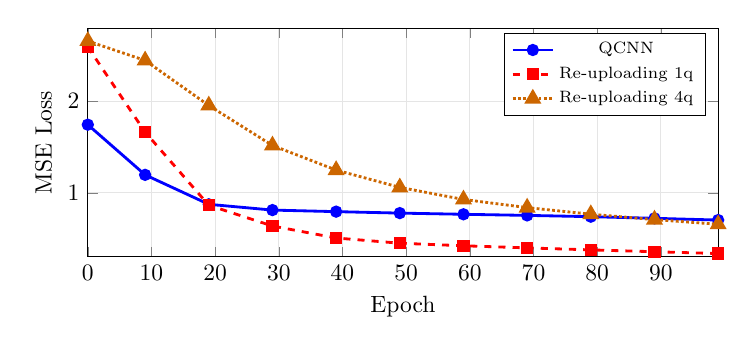
\begin{tikzpicture}[scale=0.85]
    \begin{axis}[
        xlabel={Epoch},
        ylabel={MSE Loss},
        xmin=0, xmax=99,
        ymin=0.3, ymax=2.8,
        legend style={at={(0.98,0.98)}, anchor=north east, font=\scriptsize},
        grid=major,
        grid style={gray!20},
        width=11cm, height=5cm,
    ]
    % QCNN standard (seed 0) -- solid + circle markers
    \addplot[blue, very thick, mark=*, mark size=2pt, mark options={solid, fill=blue}] coordinates {
        (0,1.745) (9,1.197) (19,0.875) (29,0.812) (39,0.795)
        (49,0.779) (59,0.766) (69,0.754) (79,0.740) (89,0.722) (99,0.703)
    };
    \addlegendentry{QCNN}

    % Re-uploading 1q standard (seed 0) -- dashed + square markers
    \addplot[red, very thick, dashed, mark=square*, mark size=2pt, mark options={solid, fill=red}] coordinates {
        (0,2.595) (9,1.664) (19,0.865) (29,0.638) (39,0.507)
        (49,0.450) (59,0.422) (69,0.399) (79,0.377) (89,0.357) (99,0.337)
    };
    \addlegendentry{Re-uploading 1q}

    % Re-uploading 4q standard (seed 0) -- dotted + triangle markers (darker orange for B&W readability)
    \addplot[orange!80!black, very thick, densely dotted, mark=triangle*, mark size=3pt, mark options={solid, fill=orange!80!black}] coordinates {
        (0,2.659) (9,2.447) (19,1.955) (29,1.518) (39,1.249)
        (49,1.060) (59,0.928) (69,0.839) (79,0.767) (89,0.708) (99,0.657)
    };
    \addlegendentry{Re-uploading 4q}
    \end{axis}
\end{tikzpicture}
\caption{Training loss curves for quantum models on the standard 3-class setting (100~epochs, 500~training samples, seed~0). All three models converge, with the single-qubit re-uploading reaching the lowest loss (0.34).}
\label{fig:loss_curves}
\end{figure}

All three quantum models show monotonically decreasing loss. The single-qubit re-uploading converges fastest, reaching a loss of 0.34 by epoch~99. The QCNN plateaus around epoch~30 and then decreases slowly to 0.70. The 4-qubit re-uploading model starts slowest but continues to improve throughout, reaching 0.66 by epoch~99.

The slower convergence of the 4-qubit model has three causes. First, its 72~parameters per classifier define a higher-dimensional loss landscape with more local minima. Second, the CZ entanglement gates create inter-qubit correlations that make individual parameter gradients less informative. Third, the averaged measurement $\langle H \rangle = \frac{1}{4}\sum_q Z_q$ dilutes the gradient signal compared to a single-qubit $\langle Z \rangle$. These effects are consistent with the barren plateau phenomenon~\cite{mcclean2018barren}.

\subsection{Ablation: Effect of Dataset Size}
\label{sec:res_ablation_data}

I investigate whether the quantum models benefit from additional training data by varying the number of training samples from 100 to 1000 (all with 100~epochs, seed~42). For datasets larger than 500~samples, I use mini-batch training (batch size 100). Table~\ref{tab:res_ablation_data} reports the resulting 3-class accuracy for each size.

\begin{table}[ht]
\centering
\begin{tabular}{lcccc}
    \toprule
    \textbf{Model} & $n=100$ & $n=250$ & $n=500$ & $n=1000$ \\
    \midrule
    Re-uploading 1q & 0.750 & 0.730 & 0.730 & 0.730 \\
    Re-uploading 4q & 0.695 & 0.700 & 0.680 & 0.700 \\
    QCNN (8q)       & 0.705 & 0.695 & 0.680 & 0.680 \\
    \midrule
    SVM (RBF)       & \multicolumn{4}{c}{0.970} \\
    Random Forest   & \multicolumn{4}{c}{0.990} \\
    \bottomrule
\end{tabular}
\caption{Standard 3-class accuracy vs.\ training set size (100~epochs, seed~42). All quantum models remain in the 68--75\% range regardless of dataset size, confirming that circuit capacity---not data---is the bottleneck.}
\label{tab:res_ablation_data}
\end{table}

All three quantum models are remarkably stable across dataset sizes (68--75\%), indicating that circuit capacity saturates with as few as 100~samples. No quantum model approaches the classical baselines. These results confirm that \emph{circuit capacity}, not training data, is the primary bottleneck for quantum classifiers on this task.

% ============================================================
\section{Discussion}
\label{sec:res_discussion}

The experiments yield three complementary findings: (i) classical baselines dominate on the standard task (99\% vs.\ 68--75\% for quantum, regardless of training budget), consistent with the expectation that quantum advantage is unlikely on classically separable data~\cite{schuld2021effect, bowles2024better}; (ii) on zero-day, supervised classical and supervised re-uploading both fail ($<3\%$ and 7--9\%), while two approaches---the unsupervised autoencoder (70.5\% $\pm$ 14.4\%, trained on normal traffic only) and the supervised QCNN excl.\ barren seeds (68.6\% $\pm$ 6.8\%, trained on normal-vs-DoS but transferring to injection)---succeed at comparable levels through very different mechanisms (reconstruction error vs.\ quantum feature separation); and (iii) the QCNN has lower variance when it trains (6.8\% vs.\ 14.4\%) but collapses 3/10 seeds vs.\ 1/10 for the autoencoder, and the 56$\times$ training-set asymmetry favours the autoencoder further. The QCNN's hierarchical pooling ($8 \to 1$) is what differentiates it from the re-uploading variants: same angle encoding, but multi-scale compression. The QCNN does not strictly dominate the autoencoder, but reaches comparable performance with 56$\times$ less training data---consistent with literature on quantum feature spaces and out-of-distribution generalization~\cite{havlicek2019supervised, schuld2020circuit}. Remaining limitations and perspectives are discussed in Chapter~\ref{chap:conclusion}.
